\documentclass{article}
\usepackage[utf8]{inputenc}
\usepackage{mathtools}
\usepackage{amssymb}
\usepackage{amsmath}
\usepackage{listings}
\usepackage{braket}
\usepackage[toc,page]{appendix}

%%%THEOREM (ETC) ENVIRONMENTS
\newtheorem{definition}{Definition}
\newtheorem{claim}{Claim}
\newtheorem{conjecture}{Conjecture}
\newtheorem{corollary}{Corollary}
\newtheorem{example}{Example}
\newtheorem{problem}{Problem}
\newtheorem{idea}{Idea} 

\usepackage{proof}
\newtheorem{theorem}{Theorem}

\newtheorem{lemma}[theorem]{Lemma}
\newtheorem{proposition}[theorem]{Proposition}

\newenvironment{proof}[1][Proof]{\begin{trivlist}
\item[\hskip \labelsep {\bfseries #1}]}{\begin{flushright}$\blacksquare$\end{flushright} \end{trivlist}}
\newenvironment{remark}[1][Remark]{\begin{trivlist}
\item[\hskip \labelsep {\bfseries #1}]}{\end{trivlist}}

\newcommand{\cat}{\mathcal{C}}
\newcommand{\Tau}{\mathrm{T}}
\newcommand{\ham}{\mathcal{H}}
\title{Hopf Algebras in Quantum Computation}
\author{Giovanni de Felice}
\date{April 2017}

%%%TIKZ:
\usepackage{tikz,pgfplots}
\usetikzlibrary{shapes.geometric}
\usetikzlibrary{trees, patterns}
\usetikzlibrary{positioning}
\usepackage{tikz,ifthen,calc}
\usepackage{tkz-euclide}
\usetikzlibrary{shapes,snakes}
\usetikzlibrary{calc,intersections, fit, knots, hobby, positioning, patterns}
\usepackage{braids}

%%%categorical diagrams:
\tikzset{
	buffer/.style={
		draw,
		shape border rotate=180,
		regular polygon,
		regular polygon sides=3,
		node distance=2cm,
		minimum height=4em
	}
}
\tikzstyle{arr}=[markings,mark=at position 0.5 with {\arrow{<}}]
%%%HOPF ALGEBRAS:
\newcommand{\mult}{
	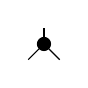
\begin{tikzpicture}[scale=0.2, black/.style={scale=0.5,draw,shape=circle,fill=black}]
	\node[black] (0) at (0, 0) {};
	\draw (1,-1) to (0);
	\draw (-1,-1) to (0);
	\draw (0) to (0,1);
	\end{tikzpicture}
}
\newcommand{\unit}{
	
\begin{tikzpicture}[scale=0.2, black/.style={scale=0.5,draw,shape=circle,fill=black}]
	\node[black] (0) at (0, 0) {};
	\draw (0) to (0,1);
	\end{tikzpicture}
}
\newcommand{\comult}{
	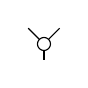
\begin{tikzpicture}[scale=0.2, black/.style={scale=0.5,draw,shape=circle,fill=white}]
	\node[black] (0) at (0, 0) {};
	\draw (1,1) to (0);
	\draw (-1,1) to (0);
	\draw (0) to (0,-1);
	\end{tikzpicture}
}

\newcommand{\counit}{
	\begin{tikzpicture}[scale=0.2, black/.style={scale=0.5,draw,shape=circle,fill=white}]
	\node[black] (0) at (0, 0) {};
	\draw (0) to (0,-1);
	\end{tikzpicture}
}

\newcommand{\antipode}{
	\begin{tikzpicture}[scale=0.2, black/.style={scale=0.5,draw,regular polygon,
		regular polygon sides=4,fill=white}]
	\node[scale=0.5, black] (0) at (0, 0) {$S$};
	\draw (0) to (0,-1);
	\draw (0) to (0,1);
	\end{tikzpicture}
}


\newcommand{\associativity}{
\begin{equation}
\begin{gathered}
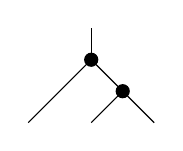
\begin{tikzpicture}[scale=0.8]
\node[scale=0.5,draw,circle,fill=black] (0) at (0,0.5) {};
\node[scale=0.5,draw,circle,fill=black] (1) at (0.5,0) {};
\draw (0) to (1);
\draw (-1,-0.5) to (0);
\draw (0,-0.5) to (1);
\draw (1,-0.5) to (1);
\draw (0) to (0,1);
\end{tikzpicture}
\end{gathered}
\, = \,
\begin{gathered}
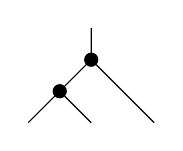
\begin{tikzpicture}[scale=0.8]
\node[scale=0.5,draw,circle,fill=black] (0) at (0.5,0.5) {};
\node[scale=0.5,draw,circle,fill=black] (1) at (0,0) {};
\draw (0) to (1);
\draw (-0.5,-0.5) to (1);
\draw (0.5,-0.5) to (1);
\draw (1.5,-0.5) to (0);
\draw (0) to (0.5,1);
\end{tikzpicture}
\end{gathered}
\end{equation}
}
\newcommand{\unitlaw}{
\begin{equation}
\begin{gathered}
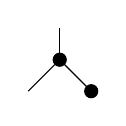
\begin{tikzpicture}[scale=0.8]
\node[scale=0.5,draw,circle,fill=black] (0) at (0,0.5) {};
\node[scale=0.5,draw,circle,fill=black] (1) at (0.5,0) {};
\draw (0) to (1);
\draw (-0.5,0) to (0);
\draw (0) to (0,1);
\end{tikzpicture}
\end{gathered}
\, = \,
\begin{gathered}
\begin{tikzpicture}[scale=0.8]
\draw (0,0) to (0,1);
\end{tikzpicture}
\end{gathered}
\, = \,
\begin{gathered}
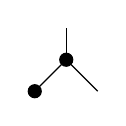
\begin{tikzpicture}[scale=0.8]
\node[scale=0.5,draw,circle,fill=black] (0) at (0,0.5) {};
\node[scale=0.5,draw,circle,fill=black] (1) at (-0.5,0) {};
\draw (0) to (1);
\draw (0.5,0) to (0);
\draw (0) to (0,1);
\end{tikzpicture}
\end{gathered}
\end{equation}
}
\newcommand{\coassociativity}{
\begin{equation}
\begin{gathered}
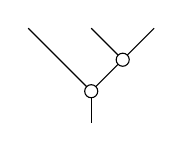
\begin{tikzpicture}[scale=0.8]
\node[scale=0.5,draw,circle,fill=white] (0) at (0,-0.5) {};
\node[scale=0.5,draw,circle,fill=white] (1) at (0.5,0) {};
\draw (0) to (1);
\draw (-1,0.5) to (0);
\draw (0,0.5) to (1);
\draw (1,0.5) to (1);
\draw (0) to (0,-1);
\end{tikzpicture}
\end{gathered}
\, = \,
\begin{gathered}
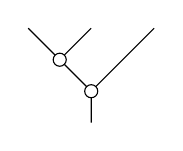
\begin{tikzpicture}[scale=0.8]
\node[scale=0.5,draw,circle,fill=white] (0) at (0.5,-0.5) {};
\node[scale=0.5,draw,circle,fill=white] (1) at (0,0) {};
\draw (0) to (1);
\draw (-0.5,0.5) to (1);
\draw (0.5,0.5) to (1);
\draw (1.5,0.5) to (0);
\draw (0) to (0.5,-1);
\end{tikzpicture}
\end{gathered}
\end{equation}
}
\newcommand{\counitlaw}{
\begin{equation}
\begin{gathered}
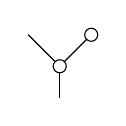
\begin{tikzpicture}[scale=0.8]
\node[scale=0.5,draw,circle,fill=white] (0) at (0,-0.5) {};
\node[scale=0.5,draw,circle,fill=white] (1) at (0.5,0) {};
\draw (0) to (1);
\draw (-0.5,0) to (0);
\draw (0) to (0,-1);
\end{tikzpicture}
\end{gathered}
\, = \,
\begin{gathered}
\begin{tikzpicture}[scale=0.8]
\draw (0,0) to (0,1);
\end{tikzpicture}
\end{gathered}
\, = \,
\begin{gathered}
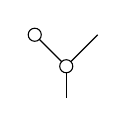
\begin{tikzpicture}[scale=0.8]
\node[scale=0.5,draw,circle,fill=white] (0) at (0,-0.5) {};
\node[scale=0.5,draw,circle,fill=white] (1) at (-0.5,0) {};
\draw (0) to (1);
\draw (0.5,0) to (0);
\draw (0) to (0,-1);
\end{tikzpicture}
\end{gathered}
\end{equation}
}

\newcommand{\bialgebralaw}{
\begin{equation}
\begin{gathered}
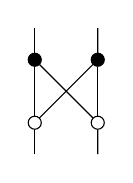
\begin{tikzpicture}[scale=0.8]
\node[scale=0.5,draw,circle,fill=white] (0) at (0,0) {};
\node[scale=0.5,draw,circle,fill=white] (1) at (1,0) {};
\node[scale=0.5,draw,circle,fill=black] (2) at (0,1) {};
\node[scale=0.5,draw,circle,fill=black] (3) at (1,1) {};
\draw (0) to (2);
\draw (0) to (3);
\draw (1) to (2);
\draw (1) to (3);
\draw (0,-0.5) to (0);
\draw (1,-0.5) to (1);
\draw (0,1.5) to (2);
\draw (1,1.5) to (3);
\end{tikzpicture}
\end{gathered}
\, = \,
\begin{gathered}
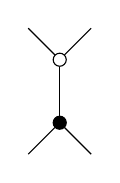
\begin{tikzpicture}[scale=0.8]
\node[scale=0.5,draw,circle,fill=black] (0) at (0.5,0) {};
\node[scale=0.5,draw,circle,fill=white] (1) at (0.5,1) {};
\draw (0) to (1);
\draw (0,-0.5) to (0);
\draw (1,-0.5) to (0);
\draw (0,1.5) to (1);
\draw (1,1.5) to (1);
\end{tikzpicture}
\end{gathered}
\end{equation}
}
\newcommand{\copylaw}{
\begin{equation}
\begin{gathered}
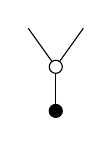
\begin{tikzpicture}[scale=0.7, squr/.style={scale=0.5,draw,regular polygon,
	regular polygon sides=4,fill=white}, black/.style={scale=0.5,draw,shape=circle,fill=black}, whit/.style={scale=0.5,draw,shape=circle,fill=white}]
\node[black] (0) at (0, 0) {};
\node[whit] (1) at  (0, 0.8) {};
\draw (0) to (1);
\draw (1) to (0.5,1.5);
\draw (1) to (-0.5,1.5);
\end{tikzpicture}
\end{gathered}
\, = \,
\begin{gathered}
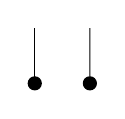
\begin{tikzpicture}[scale=0.7, black/.style={scale=0.5,draw,shape=circle,fill=black}]
\node[black] (0) at (0,0) {};
\node[black] (1) at (1,0) {};
\draw (0) to (0,1);
\draw (1) to (1,1);
\end{tikzpicture}
\end{gathered}
\end{equation}
}
\newcommand{\cocopylaw}{
	\begin{equation}
	\begin{gathered}
	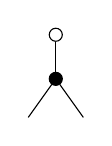
\begin{tikzpicture}[scale=0.7, squr/.style={scale=0.5,draw,regular polygon,
		regular polygon sides=4,fill=white}, black/.style={scale=0.5,draw,shape=circle,fill=black}, whit/.style={scale=0.5,draw,shape=circle,fill=white}]
	\node[whit] (0) at (0, 0) {};
	\node[black] (1) at  (0, -0.8) {};
	\draw (0) to (1);
	\draw (1) to (0.5,-1.5);
	\draw (1) to (-0.5,-1.5);
	\end{tikzpicture}
	\end{gathered}
	\, = \,
	\begin{gathered}
	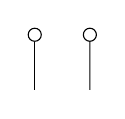
\begin{tikzpicture}[scale=0.7, black/.style={scale=0.5,draw,shape=circle,fill=white}]
	\node[black] (0) at (0,0) {};
	\node[black] (1) at (1,0) {};
	\draw (0) to (0,-1);
	\draw (1) to (1,-1);
	\end{tikzpicture}
	\end{gathered}
	\end{equation}
}
\newcommand{\hopflaw}{
	\begin{equation}
	\begin{gathered}
	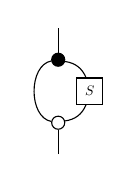
\begin{tikzpicture}[scale=0.8, squr/.style={scale=0.5,draw,regular polygon,
		regular polygon sides=4,fill=white}]
	\node[scale=0.5,draw,circle,fill=white] (0) at (0,0) {};
	\node[scale=0.5,draw,circle,fill=black] (1) at (0,1) {};
	\node[squr] (2) at (0.5,0.5) {$S$};
	\draw[bend left=80] (0) to (1);
	\draw[bend right] (0) to (2);
	\draw[bend right] (2) to (1);
	\draw (0,-0.5) to (0);
	\draw (0,1.5) to (1);
	\end{tikzpicture}
	\end{gathered}
	\, = \,
	\begin{gathered}
	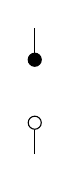
\begin{tikzpicture}[scale=0.8, squr/.style={draw,regular polygon,
		regular polygon sides=4,fill=white}]
	\node[scale=0.5,draw,circle,fill=white] (0) at (0,0) {};
	\node[scale=0.5,draw,circle,fill=black] (1) at (0,1) {};
	\draw (0,-0.5) to (0);
	\draw (0,1.5) to (1);
	\end{tikzpicture}
	\end{gathered}
	\, = \,
	\begin{gathered}
	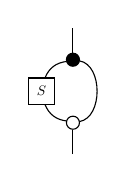
\begin{tikzpicture}[scale=0.8, squr/.style={scale=0.5,draw,regular polygon,
		regular polygon sides=4,fill=white}]
	\node[scale=0.5,draw,circle,fill=white] (0) at (0,0) {};
	\node[scale=0.5,draw,circle,fill=black] (1) at (0,1) {};
	\node[squr] (2) at (-0.5,0.5) {$S$};
	\draw[bend right=80] (0) to (1);
	\draw[bend left] (0) to (2);
	\draw[bend left] (2) to (1);
	\draw (0,-0.5) to (0);
	\draw (0,1.5) to (1);
	\end{tikzpicture}
	\end{gathered}
	\end{equation}
}
\newcommand{\modulelaw}{
	\begin{equation}
	\begin{gathered}
	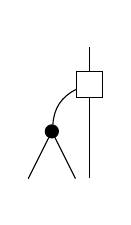
\begin{tikzpicture}[scale=0.6, squr/.style={draw,regular polygon,
		regular polygon sides=4,fill=white}, black/.style={scale=0.5,draw,shape=circle,fill=black}]
	\node (0) at (0, -2.2) {};
	\node[squr] (1) at (0, 0) {};
	\node (2) at (0, 1) {};
	\node[black] (3) at (-0.8, -1) {};
	\draw (0) to (1);
	\draw (1) to (2);
	\draw[bend left] (3) to (1);
	\draw (-1.3, -2) to (3);
	\draw (-0.3, -2) to (3);
	\end{tikzpicture}
	\end{gathered}
	\, = \,
	\begin{gathered}
	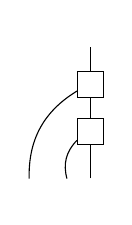
\begin{tikzpicture}[scale=0.6, squr/.style={draw,regular polygon,
		regular polygon sides=4,fill=white}, black/.style={draw,shape=circle,fill=black}]
	\node (0) at (0, -2.2) {};
	\node[squr] (1) at (0, 0) {};
	\node (2) at (0, 1) {};
	\node[squr] (3) at (0, -1) {};
	\draw (0) to (3);
	\draw (3) to (1);
	\draw (1) to (2);
	\draw (3) to (1);
	\draw[bend left] (-1.3, -2) to (1);
	\draw[bend left] (-0.5, -2) to (3);
	\end{tikzpicture}
	\end{gathered}
	\end{equation}
}
\newcommand{\comodulelaw}{
	\begin{equation}
	\begin{gathered}
	\begin{tikzpicture}[scale=0.6, squr/.style={draw,regular polygon,
		regular polygon sides=4,fill=white}, black/.style={scale=0.5,draw,shape=circle,fill=white}]
	\node (0) at (0, 2.2) {};
	\node[squr] (1) at (0, 0) {};
	\node (2) at (0, -2) {};
	\node[black] (3) at (-0.8, 1) {};
	\draw (0) to (1);
	\draw (1) to (2);
	\draw[bend right] (3) to (1);
	\draw (-1.3, 2) to (3);
	\draw (-0.3, 2) to (3);
	\end{tikzpicture}
	\end{gathered}
	\, = \,
	\begin{gathered}
	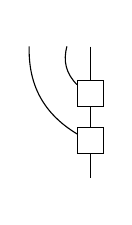
\begin{tikzpicture}[scale=0.6, squr/.style={draw,regular polygon,
		regular polygon sides=4,fill=white}, black/.style={draw,shape=circle,fill=black}]
	\node (0) at (0, 2.2) {};
	\node[squr] (1) at (0, 0) {};
	\node (2) at (0, -1) {};
	\node[squr] (3) at (0, 1) {};
	\draw (0) to (3);
	\draw (3) to (1);
	\draw (1) to (2);
	\draw (3) to (1);
	\draw[bend right] (-1.3, 2) to (1);
	\draw[bend right] (-0.5, 2) to (3);
	\end{tikzpicture}
	\end{gathered}
	\end{equation}
}
\newcommand{\intertwinerlaw}{
\begin{equation}
\begin{gathered}
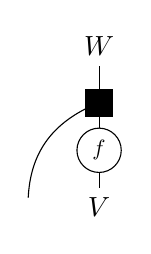
\begin{tikzpicture}[scale=0.6, squr/.style={draw,regular polygon,
	regular polygon sides=4,fill=black}]
\node (0) at (0, -2.2) {$V$};
\node[squr] (1) at (0, 0) {};
\node (2) at (0, 1.2) {$W$};
\node[scale=0.8,draw,circle] (3) at (0, -1) {$f$};
\draw (0) to (3);
\draw (3) to (1);
\draw (1) to (2);
\draw (3) to (1);
\draw[bend left] (-1.5, -2) to (1);
\end{tikzpicture}	
\end{gathered}
\, = \,
\begin{gathered}
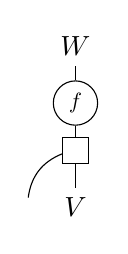
\begin{tikzpicture}[scale=0.6, squr/.style={draw,regular polygon,
	regular polygon sides=4,fill=white}]
\node (0) at (0, -2.2) {$V$};
\node[scale=0.8,draw,circle] (1) at (0, 0) {$f$};
\node (2) at (0, 1.2) {$W$};
\node[squr] (3) at (0, -1) {};
\draw (0) to (3);
\draw (3) to (1);
\draw (1) to (2);
\draw (3) to (1);
\draw[bend left] (-1, -2) to (3);
\end{tikzpicture}	
\end{gathered}
\end{equation}
}
\newcommand{\symAB}{
	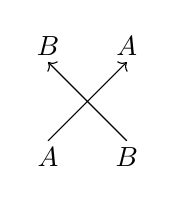
\begin{tikzpicture}[decoration={markings,mark=at position 0.5 with {\arrow{>}}}]
	\node (0) at (-0.5, -0.7) {$A$};
	\node (0) at (-0.5, 0.7) {$B$};
	\node (1) at (0.5, -0.7) {$B$};
	\node (1) at (0.5, 0.7) {$A$};
	\draw [->] (-0.5, -0.5) to (0.5, 0.5);
	\draw [->] (0.5, -0.5) to (-0.5, 0.5);
	\end{tikzpicture}
}

\newcommand{\symequation}{
	\begin{equation*}
	\begin{gathered}
	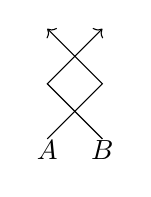
\begin{tikzpicture}[scale=0.7]
	\node (0) at (-1, -1.2) {$A$};
	\node (0) at (0, -1.2) {$B$};
	\draw [->] (-1, -1)--(0,0)--(-1,1);
	\draw [->] (0, -1)--(-1,0)--(0,1);
	\end{tikzpicture}
	\end{gathered}
	\, = \,
	\begin{gathered}
	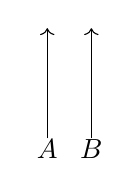
\begin{tikzpicture}[scale=0.7]
	\node (0) at (-0.8, -1.2) {$A$};
	\node (0) at (0, -1.2) {$B$};
	\draw [->] (-0.8, -1)--(-0.8,1);
	\draw [->] (0, -1)--(0,1);
	\end{tikzpicture}
	\end{gathered}
	\end{equation*}
}

\newcommand{\cupA}{	
	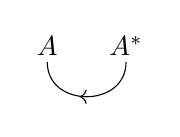
\begin{tikzpicture}[decoration={markings,mark=at position 0.5 with {\arrow{<}}}]
	\node (0) at (0, 0.2) {$A$};
	\node (1) at (1, 0.2) {$A^*$};
	\draw [bend right=90, looseness=1.5, postaction=decorate] (0,0) to (1,0);
	\end{tikzpicture}}

\newcommand{\capA}{	
	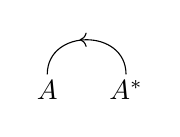
\begin{tikzpicture}[decoration={markings,mark=at position 0.5 with {\arrow{<}}}]
	\node (0) at (0, -0.2) {$A$};
	\node (1) at (1, -0.2) {$A^*$};
	\draw [bend left=90, looseness=1.5, postaction=decorate] (0,0) to (1,0);
	\end{tikzpicture}}

\newcommand{\snake}{
	\begin{equation*}
	\begin{gathered}
	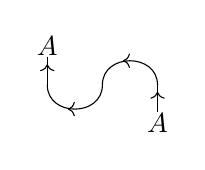
\begin{tikzpicture}[scale=0.7,decoration={markings,mark=at position 0.5 with {\arrow{<}}}]
	\node (0) at (0, 0.7) {$A$};
	\node (4) at (2, -0.7){$A$};
	\draw [bend right=90, looseness=1.5, postaction=decorate] (0, 0) to (1, 0);
	\draw [bend left=90, looseness=1.5, postaction=decorate] (1, 0) to (2, 0);
	\draw [postaction=decorate] (2, 0) to (2, -0.5);
	\draw [postaction=decorate] (0, 0.5) to (0, 0);
	\end{tikzpicture}
	\end{gathered}
	\, = \,
	\begin{gathered}
	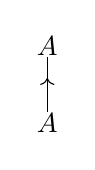
\begin{tikzpicture}[scale=0.7,decoration={markings,mark=at position 0.5 with {\arrow{<}}}]
	\node (0) at (0, 0.7) {$A$};
	\node (4) at (0, -0.7){$A$};
	\draw [postaction=decorate] (0, 0.5) to (0, -0.5);
	\end{tikzpicture}
	\end{gathered}
	\end{equation*}}

\newcommand{\snakestar}{
	\begin{equation*}
	\begin{gathered}
	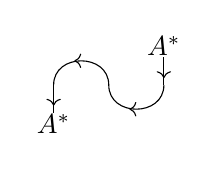
\begin{tikzpicture}[scale=0.7,decoration={markings,mark=at position 0.5 with {\arrow{<}}}]
	\node (0) at (0, -0.7) {$A^*$};
	\node (4) at (2, 0.7){$A^*$};
	\draw [bend left=90, looseness=1.5, postaction=decorate] (0, 0) to (1, 0);
	\draw [bend right=90, looseness=1.5, postaction=decorate] (1, 0) to (2, 0);
	\draw [postaction=decorate] (2, 0) to (2, 0.5);
	\draw [postaction=decorate] (0, -0.5) to (0, 0);
	\end{tikzpicture}
	\end{gathered}
	\, = \,
	\begin{gathered}
	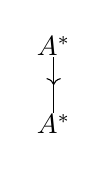
\begin{tikzpicture}[scale=0.7,decoration={markings,mark=at position 0.5 with {\arrow{>}}}]
	\node (0) at (0, 0.7) {$A^*$};
	\node (4) at (0, -0.7){$A^*$};
	\draw [postaction=decorate] (0, 0.5) to (0, -0.5);
	\end{tikzpicture}
	\end{gathered}
	\end{equation*}
}

\newcommand{\fusionijk}{
	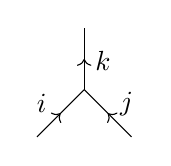
\begin{tikzpicture}[scale=0.6,decoration={markings,mark=at position 0.5 with {\arrow{>}}}]
	\node (0) at (-0.9, -0.3) {$i$};
	\node (1) at (0.9, -0.3) {$j$};
	\node (2) at (0.4, 0.6) {$k$};
	\draw [postaction=decorate] (-1, -1) to(0,0);
	\draw [postaction=decorate] (1,-1) to (0,0);
	\draw [postaction=decorate] (0,0) to (0,1.3);
	\end{tikzpicture}}
%%%%%%%%%%%%%%%%%%%%%%%%%%%%%%%%%%%%%%%%%%%%%%%%%%%%%%%%%%%%%%%%%%%%%%%%%%%%%%%%%%%%%%%%%%%%%%%%%%%%%%%%%%%%%%%%%%%%%%%%%%%%%%%%%%%%%%%%%%%%%%%%%%%%%%%%%%%%%%%%%%%%%%%%%%%%%%%%%%%%


\begin{document}

\section{Quantum Computation}

\subsection{Topological Quantum Computation}

\subsubsection{From categories to computation}
In the previous section we saw that categories can be interpreted as physical process theories. In a very similar way, we can interpret objets as data types and morphisms as computational processes, so that any category corresponds to a theory of computation. Monoidal categories are ones where parallel computation is possible. Quantum computation is a model in which data is encoded in the state of quantum systems and processes are quantum evolutions of the system. A computation consists of the preparation of some quantum states, their manipulation and measurement. Usually this procedure is repeated in order to collect statistics and approximate density distributions. The unit of information in quantum computation is called qubit by analogy with the classical bit. A qubit is a two-level quantum system, that is a Hilbert space of dimension $2$ which is denoted by $\mathbb{C}^2$. Similarly a qudit is a $d$ dimensional system $\mathbb{C}^d$.\\
Modular categories are models for topological quantum computation (TQC) in the sense of \cite{Kitaev03} or \cite{Rowell17}. TQC has been studied extensively in recent years as it allows for fault-tolerant quantum computation. In this model data is encoded in non-abelian anyons and quantum gates are obtained by braiding those particles. Topologically equivalent braids implement the same quantum process so that small perturbations of particle world-lines do not affect the computation and gates (and quantum information) are topologically protected from decoherence.
Another reason for studying topological quantum computation is that some TQC models allow to approximate the Jones polynomial in polynomial time, a problem that is believed to be untractable classically.\\
The problem of building a topological quantum computer has been addressed by various authors \cite{Kitaev03} [cite freedman]. Non-abelian anyons have never been achieved experimentally, much of the difficulty arises in the two-dimensional nature of anyons.\\
A topological quantum computer runs as follows \cite{Rowell17}:
\begin{definition}[TQC]
	\begin{enumerate}
		\item Creation of anyon pairs from the vacuum to encode the information as a quantum state.
		\item Braiding those anyons performs a quantum gate on the state.
		\item fusing neighbouring anyons and observing the resulting anyon type corresponds to a projective measurement on the system.
	\end{enumerate}
\end{definition}
The computation result is the approximation to a probability distribution (over measurement outcomes) obtained by repeating the procedure polynomially many times and recording the output anyon types. Note that if we postselct on the vacuum sector to be the output anyon type we are effetively approximating an invariant of links. Indeed any process in TQC starting and ending in the vacuum sector is a link, formed by the particle trajectories in space-time (i.e the briading process). The operations we can perform on a system $V$ are unitaries, so that any braiding process on $n$ particles induces the evaluation of some unitary representation $\beta \rightarrow U_\beta$ of the braid group $B_n$.\\
In order to make sure the braiding process is a unitary transformation of the state space we will assume one further constraint on our categorical model of computation: unitarity of the braids in the modular category in question.\\
\begin{definition}[UMC]
	A unitary modular category (UMC) is a modular category where each component of the braiding is a unitary.
\end{definition}
Given a UMC $\cat$, we have a finite set of data types $I$ given by the isomorphism classes of simple objects in $\cat$. The topological qudit is usually encoded in some fusion space as follows. We usually fix some data type $a$ and consider the fusion of $n$ copies of $a$. We then choose some output type $b$ on which to post-select in order to obtain a fusion space $V := V_{a^{\otimes n}}^b = Hom(a^{\otimes n}, b)$ of dimension $d$. We can picture standard basis as labelled binary fusion trees with $b$ at the root and $a$ on the $n$ leaves. Each binary tree shape (with $n$ leaves) corresponds to a different bracketing of $a^{\otimes n}$ and usually yields distinct bases related to each other via $F$-moves. Braiding a pair of type $a$ anyons before fusing is an $R$-move. All computational processes on $V$ can be decomposed in sequences of $F$-moves (re-bracketing) and $R$-moves (braiding).

\begin{example}[Fibonacci anyons]
	We now look back at example [ref] on Fibonacci anyons and show how to compute in the model.
	Recall we have only two particle types: the vacuum sector $1$ and the non-trivial $\tau$ such that:
	$$\tau \otimes \tau = 1 \oplus \tau$$
	$\tau$ and $1$ are their own anti-particles so we don't need to distinguish particles and antiparticles by wrinting arrows on wires.
	We can write the basis of the two dimensional space $\tau \otimes \tau$ as:
	\begin{center}
		\begin{tikzpicture}
		\node (0) at (0.3, 0.3) {$\tau$};
		\node (0) at (-0.7, -0.3) {$\tau$};
		\node (0) at (0.7, -0.3) {$\tau$};
		\draw (-0.5, -0.5)--(0,0)--(0,0.5);
		\draw (0.5, -0.5)--(0,0);
		\end{tikzpicture}
		\quad
		\begin{tikzpicture}
		\node (0) at (0.3, 0.3) {$1$};
		\node (0) at (-0.7, -0.3) {$\tau$};
		\node (0) at (0.7, -0.3) {$\tau$};
		\draw (-0.5, -0.5)--(0,0)--(0,0.5);
		\draw (0.5, -0.5)--(0,0);
		\end{tikzpicture}
	\end{center}
	The fusion space $V_{\tau^{\otimes 3}}^\tau$ is two dimensional, we will take it as our computational space. Practically, this corresponds to considering three $\tau$ particles with overall charge (type) $\tau$. This space is our topological qubit and we write the computational basis as:
	\begin{center}
		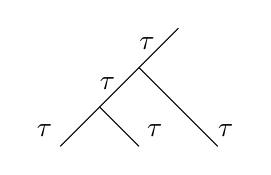
\begin{tikzpicture}
		\node (0) at (0.1, 0.3) {$\tau$};
		\node (0) at (-0.7, -0.3) {$\tau$};
		\node (0) at (0.7, -0.3) {$\tau$};
		\node (0) at (0.6, 0.8) {$\tau$};
		\node (0) at (1.6, -0.3) {$\tau$};
		\draw (-0.5, -0.5)--(0,0)--(0.5,0.5)--(1,1);
		\draw (0.5, -0.5)--(0,0);
		\draw (1.5, -0.5)--(0.5,0.5);
		\end{tikzpicture}
		\quad
		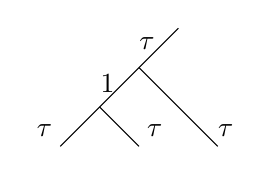
\begin{tikzpicture}
		\node (0) at (0.1, 0.3) {$1$};
		\node (0) at (-0.7, -0.3) {$\tau$};
		\node (0) at (0.7, -0.3) {$\tau$};
		\node (0) at (0.6, 0.8) {$\tau$};
		\node (0) at (1.6, -0.3) {$\tau$};
		\draw (-0.5, -0.5)--(0,0)--(0.5,0.5)--(1,1);
		\draw (0.5, -0.5)--(0,0);
		\draw (1.5, -0.5)--(0.5,0.5);
		\end{tikzpicture}
	\end{center}
	Let's denote by $\ket{0}, \ket{1}$ these basis states. Another basis is given by fusing the left-most two anyons first:
	\begin{center}
		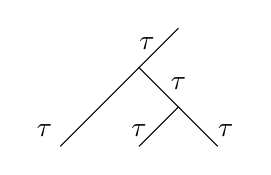
\begin{tikzpicture}
		\node (0) at (1, 0.3) {$\tau$};
		\node (0) at (-0.7, -0.3) {$\tau$};
		\node (0) at (0.5, -0.3) {$\tau$};
		\node (0) at (0.6, 0.8) {$\tau$};
		\node (0) at (1.6, -0.3) {$\tau$};
		\draw (-0.5, -0.5)--(0,0)--(0.5,0.5)--(1,1);
		\draw (0.5, -0.5)--(1,0);
		\draw (1.5, -0.5)--(0.5,0.5);
		\end{tikzpicture}
		\quad
		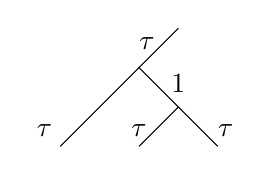
\begin{tikzpicture}
		\node (0) at (1, 0.3) {$1$};
		\node (0) at (-0.7, -0.3) {$\tau$};
		\node (0) at (0.5, -0.3) {$\tau$};
		\node (0) at (0.6, 0.8) {$\tau$};
		\node (0) at (1.6, -0.3) {$\tau$};
		\draw (-0.5, -0.5)--(0,0)--(0.5,0.5)--(1,1);
		\draw (0.5, -0.5)--(1,0);
		\draw (1.5, -0.5)--(0.5,0.5);
		\end{tikzpicture}
	\end{center}
	And we denote them by $\ket{+}, \ket{-}$. These two bases are linked by a unitary $2 \times 2$ transformation $F:= F^\tau_{\tau^{\otimes 3}}$ given by the solution of the following system:
	$$ \ket{0} = F_{0+} \ket{+} + F_{0-} \ket{-}$$
	$$ \ket{1} = F_{1+} \ket{+} + F_{1-} \ket{-}$$
	To derive the form of the $F$-matrix we need to consider the pentagon axiom. It turns out that for the Fibonacci model the pentagon is enough to derive the $F$-matrix but it is not the case in general. The resulting $F$-matrix is \cite{Simon16}:
	\begin{equation}
		 F^\tau_{\tau^{\otimes 3}} =
		\begin{bmatrix}
		\phi^{-1} & \phi^{-\frac{1}{2}} \\
		\phi^{-\frac{1}{2}} & -\phi^{-1}
		\end{bmatrix}
	\end{equation}
	where $\phi = \frac{\sqrt{5}-1}{2}$. Given the $F$-matrix and the two hexagon axioms for braided monoidal categories the possibilities for the $R$-matrix are few. In this case there is only one possibility and we obtain the $R$-matrix:
	\begin{equation}
		R^\tau_{\tau^{\otimes 3}} = 
		\begin{bmatrix}
		e^{-4\pi i/ 5} & 0 \\
		0 & -e^{-2\pi i/ 5} 
		\end{bmatrix}
	\end{equation}
	In \cite{Panangaden11} it is shown that the Fibonacci model allows universal quantum computation. This is done by first noting that polynomially many $R$ and $F$ matrices as above can approximate any unitary on one qubit, and then by constructing a CNOT gate on two topological qubits.
\end{example}

\subsubsection{Kitaev's quantum double model}
The models which we present here have first been introduced by Kitaev \cite{Kitaev03} and some special cases have been implemented experimentally on two dimensional materials at very low temperatures.\\
Suppose we have particles living in state space $H$ where $H$ is a Hopf algebra (with black multiplication, white comultiplication and antipode $S$ as usual). We can define two canonical types of left $H$-module structures on $H$ given by the right and left multiplication as follows:
\begin{equation}\label{Lmoduleaction}
	L_+ =
	\begin{gathered}
	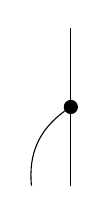
\begin{tikzpicture}
	\node[scale=0.5, draw, circle, fill=black] (0) at (0,0) {};
	\draw (0,-1)--(0)--(0,1);
	\draw [bend left] (-0.5,-1) to (0);
	\end{tikzpicture}
	\end{gathered}
	\quad ; \quad
	L_- =
	\begin{gathered}
	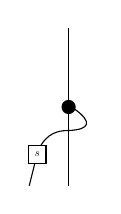
\begin{tikzpicture}[whit/.style={draw,regular polygon,
		regular polygon sides=4,fill=white}]
	\node[scale=0.5, draw, circle, fill=black] (0) at (0,0) {};
	\node[scale=0.4, whit] (s) at (-0.4,-0.6) {$s$};
	\draw (0,-1)--(0)--(0,1);
	\draw (-0.5,-1) to (s);
	\draw [bend left] (s) to (0,-0.3);
	\draw [bend right=70, looseness=2.5] (0,-0.3) to (0);
	\end{tikzpicture}
	\end{gathered}
\end{equation}
Right multiplication defines a module by associativity, left multiplication also works because the antipode is an antialgebra morphism:
\begin{equation}
	\begin{gathered}
	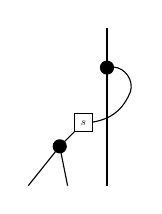
\begin{tikzpicture}[whit/.style={draw,regular polygon,
		regular polygon sides=4,fill=white}]
	\node[scale=0.5, draw, circle, fill=black] (0) at (0,0.5) {};
	\node[scale=0.5, draw, circle, fill=black] (1) at (-0.6,-0.5) {};
	\node[scale=0.4, whit] (s) at (-0.3,-0.2) {$s$};
	\draw (0,-1)--(0)--(0,1);
	\draw[bend right] (s) to (0.3,0.2);
	\draw [bend right=50] (0.3,0.2) to (0);
	\draw (-0.5,-1)--(1)--(s);
	\draw (-1,-1)--(1);
	\end{tikzpicture}
	\end{gathered}
	\, = \,
	\begin{gathered}
	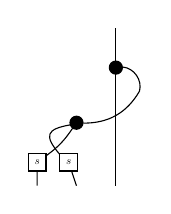
\begin{tikzpicture}[whit/.style={draw,regular polygon,
		regular polygon sides=4,fill=white}]
	\node[scale=0.5, draw, circle, fill=black] (0) at (0,0.5) {};
	\node[scale=0.5, draw, circle, fill=black] (1) at (-0.5,-0.2) {};
	\node[scale=0.4, whit] (s1) at (-0.6,-0.7) {$s$};
	\node[scale=0.4, whit] (s2) at (-1,-0.7) {$s$};
	\draw (0,-1)--(0)--(0,1);
	\draw[bend right] (1) to (0.3,0.2);
	\draw [bend right=50] (0.3,0.2) to (0);
	\draw (-0.5,-1)--(s1);
	\draw (-1,-1)--(s2);
	\draw [bend left=60,looseness=2] (s1) to (1); 
	\draw[bend right=10] (s2) to (1);
	\end{tikzpicture}
	\end{gathered}
	\, = \,
	\begin{gathered}
	\begin{tikzpicture}[whit/.style={draw,regular polygon,
		regular polygon sides=4,fill=white}]
	\node[scale=0.5, draw, circle, fill=black] (0) at (0,0.5) {};
	\node[scale=0.5, draw, circle, fill=black] (1) at (0,-0.2) {};
	\node[scale=0.4, whit] (s1) at (-0.4,-0.7) {$s$};
	\node[scale=0.4, whit] (s2) at (-1,-0.7) {$s$};
	\draw (0,-1)--(1)--(0)--(0,1);
	\draw [bend left] (s2) to (0,0.2);
	\draw [bend right=70, looseness=2] (0,0.2) to (0);
	\draw (-0.5,-1)--(s1);
	\draw (-1,-1)--(s2);
	\draw [bend left] (s1) to (0,-0.5);
	\draw [bend right=70, looseness=2] (0,-0.5) to (1); 
	\end{tikzpicture}
	\end{gathered}
\end{equation}
Similarly there are two canonical left $H$-comodule structures on $H$ given by left and right comultiplication.
\begin{equation}\label{Tmodulecoaction}
	T_+ =
	\begin{gathered}
	\begin{tikzpicture}
	\node[scale=0.5, draw, circle, fill=white] (0) at (0,0) {};
	\draw (0,-1)--(0)--(0,1);
	\draw [bend right] (-0.5,1) to (0);
	\end{tikzpicture}
	\end{gathered}
	\quad ; \quad
	T_- =
	\begin{gathered}
	\begin{tikzpicture}[whit/.style={draw,regular polygon,
		regular polygon sides=4,fill=white}]
	\node[scale=0.5, draw, circle, fill=white] (0) at (0,0) {};
	\node[scale=0.4, whit] (s) at (-0.4,0.6) {$s$};
	\draw (0,-1)--(0)--(0,1);
	\draw (-0.5,1) to (s);
	\draw [bend right] (s) to (0,0.3);
	\draw [bend left=70, looseness=2.5] (0,0.3) to (0);
	\end{tikzpicture}
	\end{gathered}
\end{equation}
And the proofs that these are $H$-comodules are dual to the previous ones.
Kitaev considers the case where $H=\mathbb{C}G$ for some group $G$. The above module and comdule structures then yield 4 types of linear operators on $\mathbb{C}G$: $L^g_\pm$, $T^h_\pm$ (using the notation from \cite{Kitaev03}), indexed by elements $g,h \in G$, and defined as follows:
\begin{equation}
	\begin{aligned}
	L^g_+ \ket{z} = \ket{gz} \quad& L^g_- \ket{z} = \ket{zg^{-1}}\\
	T^h_+ \ket{z} = \delta_{h,z} \ket{z} \quad& T^h_- \ket{z} = \delta_{h^{-1},z} \ket{z}
	\end{aligned}	 
\end{equation}
Note that $L$ operators commute with each other and $T$ operators too. The non-trivial commutation relations are the following:
\begin{equation}
	\begin{aligned}
	L^g_+ T^h_+ = T^{gh}_+ L^g_+ &\quad L^g_+ T^h_- = T^{hg^{-1}}_- L^g_+ \\
	L^g_- T^h_+ = T^{hg^{-1}}_+ L^g_- &\quad L^g_- T^h_- = T^{gh}_- L^g_-
	\end{aligned} 
\end{equation}
In the general Hopf algebra case those commutation relations correspond to the following equalities of diagrams, which are easily obtained using the bialgebra rule and the fact that the antipode is an anti-algebra and an anti-coalgebra morphism.
\begin{equation}\label{l+t+}
	\begin{gathered}
	\begin{tikzpicture}
	\node[scale=0.5, draw, circle, fill=white] (w) at (0,0.5) {};
	\node[scale=0.5, draw, circle, fill=black] (b) at (0,-0.5) {};
	\draw (0,-1)--(b)--(w)--(0,1);
	\draw [bend right] (-0.5,1) to (w);
	\draw [bend left] (-0.5,-1) to (b);
	\end{tikzpicture}
	\end{gathered}
	\, = \,
	\begin{gathered}
	\begin{tikzpicture}
	\node[scale=0.5, draw, circle, fill=black] (w1) at (0,0.5) {};
	\node[scale=0.5, draw, circle, fill=white] (b1) at (0,-0.5) {};
	\node[scale=0.5, draw, circle, fill=black] (w2) at (-0.5,0.5) {};
	\node[scale=0.5, draw, circle, fill=white] (b2) at (-0.5,-0.5) {};
	\draw (0,-1)--(b1)--(w1)--(0,1);
	\draw (-0.5,1)--(w2)--(b1);
	\draw (-0.5,-1)--(b2)--(w1);
	\draw (b2)--(w2);
	\end{tikzpicture}
	\end{gathered}
\end{equation}
\begin{equation}\label{l+t-}
\begin{gathered}
\begin{tikzpicture}[whit/.style={draw,regular polygon,
	regular polygon sides=4,fill=white}]
\node[scale=0.5, draw, circle, fill=white] (w) at (0,0) {};
\node[scale=0.5, draw, circle, fill=black] (b) at (0,-0.5) {};
\node[scale=0.4, whit] (s) at (-0.4,0.6) {$s$};
\draw (0,-1)--(b)--(w)--(0,1);
\draw (-0.5,1) to (s);
\draw [bend right] (s) to (0,0.3);
\draw [bend left=70, looseness=2.5] (0,0.3) to (w);
\draw [bend left] (-0.5,-1) to (b);
\end{tikzpicture}
\end{gathered}
\, = \,
\begin{gathered}
\begin{tikzpicture}[whit/.style={draw,regular polygon,
	regular polygon sides=4,fill=white}]
\node[scale=0.5, draw, circle, fill=white] (w) at (0,-0.5) {};
\node[scale=0.5, draw, circle, fill=black] (b) at (0,0.5) {};
\node[scale=0.5, draw, circle, fill=white] (w2) at (-0.5,-0.8) {};
\node[scale=0.5, draw, circle, fill=black] (b2) at (-0.5,0.8) {};
\node[scale=0.4, whit] (s) at (-0.5,0.4) {$s$};
\node[scale=0.4, whit] (s2) at (0.5,0) {$s$};
\draw (0,-1)--(w)--(b)--(0,1);
\draw (-0.5,1)--(b2)--(s);
\draw [bend right] (s) to (0,-0.2);
\draw [bend left=70, looseness=2.5] (0,-0.2) to (w);
\draw (-0.5,-1)--(w2);
\draw [bend left] (w2) to (b);
\draw [bend right=50] (w2) to (s2);
\draw [bend right=50] (s2) to (b2);
\end{tikzpicture}
\end{gathered}
\end{equation}
\begin{equation}\label{l-t+}
\begin{gathered}
\begin{tikzpicture}[whit/.style={draw,regular polygon,
	regular polygon sides=4,fill=white}]
\node[scale=0.5, draw, circle, fill=black] (w) at (0,0) {};
\node[scale=0.5, draw, circle, fill=white] (b) at (0,0.5) {};
\node[scale=0.4, whit] (s) at (-0.4,-0.6) {$s$};
\draw (0,1)--(b)--(w)--(0,-1);
\draw (-0.5,-1) to (s);
\draw [bend left] (s) to (0,-0.3);
\draw [bend right=70, looseness=2.5] (0,-0.3) to (w);
\draw [bend right] (-0.5,1) to (b);
\end{tikzpicture}
\end{gathered}
\, = \,
\begin{gathered}
\begin{tikzpicture}[whit/.style={draw,regular polygon,
	regular polygon sides=4,fill=white}]
\node[scale=0.5, draw, circle, fill=black] (w) at (0,0.5) {};
\node[scale=0.5, draw, circle, fill=white] (b) at (0,-0.5) {};
\node[scale=0.5, draw, circle, fill=black] (w2) at (-0.5,0.8) {};
\node[scale=0.5, draw, circle, fill=white] (b2) at (-0.5,-0.8) {};
\node[scale=0.4, whit] (s) at (-0.5,-0.4) {$s$};
\node[scale=0.4, whit] (s2) at (0.5,0) {$s$};
\draw (0,1)--(w)--(b)--(0,-1);
\draw (-0.5,-1)--(b2)--(s);
\draw [bend left] (s) to (0,0.2);
\draw [bend right=70, looseness=2.5] (0,0.2) to (w);
\draw (-0.5,1)--(w2);
\draw [bend right] (w2) to (b);
\draw [bend left=50] (w2) to (s2);
\draw [bend left=50] (s2) to (b2);
\end{tikzpicture}
\end{gathered}
\end{equation}
\begin{equation}\label{l-t-}
\begin{gathered}
\begin{tikzpicture}[whit/.style={draw,regular polygon,
	regular polygon sides=4,fill=white}]
\node[scale=0.5, draw, circle, fill=black] (w) at (0,-0.2) {};
\node[scale=0.5, draw, circle, fill=white] (b) at (0,0.2) {};
\node[scale=0.4, whit] (s) at (-0.4,-0.7) {$s$};
\node[scale=0.4, whit] (s2) at (-0.4,0.7) {$s$};
\draw (0,1)--(b)--(w)--(0,-1);
\draw (-0.5,-1) to (s);
\draw [bend left] (s) to (0,-0.4);
\draw [bend right=70, looseness=2.5] (0,-0.4) to (w);
\draw (-0.5,1) to (s2);
\draw [bend right] (s2) to (0,0.4);
\draw [bend left=70, looseness=2.5] (0,0.4) to (b);
\end{tikzpicture}
\end{gathered}
\, = \,
\begin{gathered}
\begin{tikzpicture}[whit/.style={draw,regular polygon,
	regular polygon sides=4,fill=white}]
\node[scale=0.5, draw, circle, fill=black] (w) at (0,0.5) {};
\node[scale=0.5, draw, circle, fill=white] (b) at (0,-0.5) {};
\node[scale=0.5, draw, circle, fill=black] (b2) at (-0.5,0.8) {};
\node[scale=0.5, draw, circle, fill=white] (w2) at (-0.5,-0.8) {};
\node[scale=0.4, whit] (s) at (-0.3,-0.4) {$s$};
\node[scale=0.4, whit] (s2) at (-0.3,0.4) {$s$};
\node[scale=0.4, whit] (s3) at (-0.8,-0.2) {$s$};
\node[scale=0.4, whit] (s4) at (-0.8,0.2) {$s$};
\draw (0,1)--(w)--(b)--(0,-1);
\draw (-0.5,-1)--(w2)--(s);
\draw [bend left] (s) to (0,0.2);
\draw [bend right=70, looseness=2.5] (0,0.2) to (w);
\draw (-0.5,1)--(b2)--(s2);
\draw [bend right] (s2) to (0,-0.2);
\draw [bend left=70, looseness=2.5] (0,-0.2) to (b);
\draw [bend left] (w2) to (s3);
\draw (s3)--(s4);
\draw [bend left] (s4) to (b2);
\end{tikzpicture}
\end{gathered}
\end{equation}
We then consider a lattice with oriented edges embedded in some $2D$ oriented manifold (e.g a sphere or a torus) with particles on the edges. For any vertex $s$ and adjacent plaquette $p$, a site is defined as the pair $a=(s,p)$. Let $star(a)$ be the set of edges adjacent to $s$ and $bound(p)=\{j_1, .. j_k\}$ the ordered set of edges adjacent to plaquette $p$ starting and ending at vertex $s$. Every edge $j \in star(s)$ on the lattice has an orientation and in \cite{Kitaev03} is defined $L^g(j,s)$ to be $L^g_-$ applied to vertex $j$ when $s$ is the origin of $j$ and $L^g_+$ otherwise. Similarly $T^h(j,p)$ is defined to be $T^h_+$ (repectively $T^h_-$) if $j$ is on the right (resp. on the left) of $j$. The following operators are then defined at each site $a$ of the lattice:
\begin{equation}\label{doubleonsite}
	\begin{aligned}
	A_g(a) &= \prod_{j \in star(s)} L^g(j,s) \\
	P_h(a) &= \sum_{h_1...h_k=h} \prod_{m=1}^{k} T^{h_m}(j_m,p)
	\end{aligned}
\end{equation}
We will write the general diagrammatic form of these operators in the next section. For the moment let us go through Kitaev's reasoning \cite{Kitaev03}.\\
From a physical point of view $P_h$ operators can be understood as measuring the magnetic flux of the system at some site and $A_g$ are local symmetry transformations on the charge. Flux measurements are projection $P_h \in \mathbb{C}G^*$ onto flux sector $h$. The allowed residual global symmetry transformations are then implemented via $A_g$ for $g \in N(h)$. \\
The projectors form a Von Neumann family and satisfy 
$$P_hP_{h'}= \delta_{h,h'} P_h.$$ 
Operators $A_g$ are global symmetry transformation 
$$A_gA_h = A_gh$$
and affect the fluxes via conjugation:
\begin{equation}\label{doublemult}
A_gP_h = P_{ghg^{-1}}A_g
\end{equation}
(this was shown was shown by Kitaev \cite{Kitaev03}). Operators $A_g$ and $P_h$ generate the algebra $DG$. So the quantum double construction allows to capture both global symmetry transformations and projective measurements in one algebraic structure. It is easy to check, rewriting the definition, that the following is true. 
\begin{proposition}
	For any finite group $G$, its quantum double $D(G)$ is the algebra generated by $\{P_hA_g\}_{h,g\in G}$ with multiplication induced by (\ref{doublemult}), comultiplication and antipode as defined in [first section]. 
\end{proposition}
$D(G)$ has a natural quasi-triangular structure witnessed by the universal R-matrix $R=\sum_{g,h \in G}P_he \otimes P_hg$, making $RepDG$ braided.\\
Kitaev then builds a Hamiltonian for the system and shows that the ground state of the Hamiltonian is an irreducible representations of $DG$. Here we will skip this part of the reasoning and rely on the intuition that the operators $A_g$ and $P_h$ correspond to the symmetries of the system, i.e the dynamics which are `constantly being applied'. So the allowed processes of the systems are processes that commute with all of those operators, i.e the system lives in a representation of $DG$. The ground state of the Hamiltonian has degeneracy $4^g$ where $g$ is the genus of the surface in which we embedded the lattice.\\
In the case of a sphere, $g=0$, so there is no degeneracy and the overall system lives in a one dimensional (trivial) representation of $DG$, the vacuum sector. An excitation can arise at some site on the lattice when the constraints given by the Hamiltonian are violated. In representation theoretic terms this corresponds to the creation of a state of some higher dimensional irreducible representation of $DG$. Those excitations (or quasi-particles) are anyons and can only be created in pairs (particle-antiparticle pairs). When the lattice is `layered' enough (i.e contains many particles) we can move those excitations on the lattice (practically this is done by applying charge and flux operators at given sites on the lattice). All the excitations can then be fused pairwise to end back in the vacuum sector and obtain fusion results. There are different possible types of excitations (anyon flavours) we can create on the lattice, corresponding to different possible violations of the constraints. These are precisely indexed by the irreducible representations of $DG$. We can see that we have obtained a physical setting giving rise to anyons whose behaviour is modeled by the modular category $Rep(DG)$.\\
In order to understand the possible anyon types in the model, we must study the irreducible representations of the quantum double finite group algebra $DG$. This has been done by Gould \cite{Gould93}, who showed that irreducible representations of $DG$ are obtained in the following way.\\
Let $\{C_i\}_{i=1}^n$ be the distinct conjugacy classes in $G$. To each of those conjugacy classes corresponds a centralizer subgroup $N_i$ (two choices of representatives for $C_i$ yield isomorphic centralizer subgroups). Then for any irreducible representation $(\alpha,V^i_\alpha)$ of $N_i$ with basis elements $v^\alpha_j$, let $V_{i,\alpha} = \mathbb{C}C_i \otimes V^i_\alpha$, this has basis $\{ \ket{k,v^\alpha_j} \}_{j=1,...,dim\alpha}^{k\in C_i}$ and forms an irreducible representation of $D(G)$ under the action 
\begin{equation}
P_hg\ket{k,v^\alpha_j} = \delta_{h,gkg^{-1}} \ket{h,\alpha(h^{-1}gk)v^\alpha_j}
\end{equation}
and the $\{V_{i,\alpha}\}$ is the complete set of irreducible representations. When $G$ is abelian, all irreducible representations are one-dimensional and we only have abelian anyons which are very unlikely to be universal for quantum computation. It was shown by Kitaev that if $G=S_5$ the model is universal for quantum computation. In [cite Lahtinen] the $G=S_3$ model was considered but not shown to be universal.
\begin{example}[Quantum memory]
	The case where $G \simeq \mathbb{Z}_2$ gives rise to Kitaev's toric code. Note that $D(\mathbb{Z}_2) \simeq \mathbb{C}(\mathbb{Z}_2\times \mathbb{Z}_2^\star)$, so that there are $4$ irreducible representations, all of which are 1-dimensional. Each of those corresponds to a different type of excitation.  Let $x$ and $y$ be the generators of the group. The trivial representation is the trivial excitation (or `no excitation'). The other irreducible representations are obtained by mapping $x$ and $y$ to order $2$  elements of $\mathbb{C}$. We obtain two bosons, when both get sent to $-1$ or $i$ and one fermions when $x \mapsto -1$ and $y \mapsto i$.\\
	If we implement the construction on a lattice embedded on a torus, we obtain a model for a topologically protected quantum memory. Consider a (layered enough) lattice on a torus with spins on the edges. Let $C_1$ and $C_2$ be two cycles. States of the system are generated by labellings of the lattice with elements of $\mathbb{Z}_2$. As shown by Kitaev, the ground state degeneracy has dimension $4$, so that we can think of the system as storing two qubits of information. If a particle-antiparticle pair is created at some site on the lattice it will re annihilate at some other site. The world-lines will form a loop on the torus and we have three possible behaviours. If the loop can be shrinked to a point, this won't affect the underlying information otherwise we obtain two non-trivial operations $T_1$ and $T_2$ affecting the ground state when the world-lines loop around cycle $C_1$ and $C_2$. If we initialise the lattice in some ground state it will remain in that state unless a $T_1$ or $T_2$ operation is implemented. If the lattice is layered enough, it is very unlikely that such processes occur spontaneously, and therefore the quantum information is protected.
\end{example}

\subsubsection{Generalising the model}
We will now try to generalize the above construction to the cases where the Hopf algebra $H$ is not a group algebra. We will wait before 'bending cables' (i.e using the dual hopf algebra) to see how far we can go without making too many assumptions on $H$. This will provide an interesting illustration of the proof given in the previous chapter [ref section]. Interpreted in this physical context, the Drinfeld construction can be understood as imposing global (or topological) dependencies on the particles under consideration (e.g in  the form of a Hamiltonian as the one considered by Kitaev) giving rise to anyonic behaviour.\\
As above, we have an oriented lattice on a $2D$ oriented manifold with particles on the edges taking values in $H$. For simplicity we will assume the manifold is a sphere and that the lattice has no loops. 
Let $\mathcal{L}_a$ be the state space of particles at some site $a=(s,p)$ (i.e the particles on edges adjacent to $s$ or $p$ with some order that we give below). We will define a left $H$-module and a left $H$-comodule structure on $\mathcal{L}_a$ and show those satisfy the left-left Yetter-Drinfeld module compatibility condition.\\
Analogously to \cite{Kitaev03} we first define an $H$-module structure $L$, for $j \in star(s) \cup bound(p)$ given by $L_-$ from (\ref{Lmoduleaction}) if $s$ is the origin of $j \in star(s)$, by $L_+$ if $j$ is not the origin and $j \in star(s)$ and the trivial $H$-module otherwise. The $H$-comodule structure is given by the $T_+$ action from (\ref{Tmodulecoaction}) if $p$ is on the right of $j$, by $T_-$ if it is on the left and by the trivial $H$-comodule otherwise. In his model, Kitaev only needed to order the edges in $bound(p)$ because the comultiplication of $\mathbb{C}G$ is just the copy map, here we will need some more conventions on the ordering of the edges.\\
We have $bound(p)= \{j_1, j_2,..., j_k\}$ starting and ending at vertex $s$, then order $star(s)=\{i_1, i_2, ..., i_n\}$ where $i_1=j_1$ and $i_n=j_k$ also note that we have $4$ possible configurations of vertex $s$ adjacent to plaquette $p$ and we can choose which of the edges is $j_1$ and which is $j_k$. We choose as follows:
\begin{center}
	\begin{tikzpicture}[decoration={markings,mark=at position 0.5 with {\arrow{>}}}]
		\node at (-0.1,0.2) {$s$};
		\node at (0.2,-0.5) {$p$};
		\node at (-0.6, -0.3) {$j_1$};
		\node at (0.6, 0.2) {$j_k$};
		\draw[postaction=decorate] (0,0)--(0.8,0);
		\draw[postaction=decorate] (0,0)--(-0.6,-0.6);
	\end{tikzpicture}
	\quad
	\begin{tikzpicture}[decoration={markings,mark=at position 0.5 with {\arrow{>}}}]
	\node at (-0.1,0.2) {$s$};
	\node at (0.2,-0.5) {$p$};
	\node at (-0.6, -0.3) {$j_k$};
	\node at (0.6, 0.2) {$j_1$};
	\draw[postaction=decorate] (0,0)--(0.8,0);
	\draw[postaction=decorate] (-0.6,-0.6)--(0,0);
	\end{tikzpicture}
	\quad
	\begin{tikzpicture}[decoration={markings,mark=at position 0.5 with {\arrow{>}}}]
	\node at (-0.1,0.2) {$s$};
	\node at (0.2,-0.5) {$p$};
	\node at (-0.6, -0.3) {$j_1$};
	\node at (0.6, 0.2) {$j_k$};
	\draw[postaction=decorate] (0.8,0)--(0,0);
	\draw[postaction=decorate] (-0.6,-0.6)--(0,0);
	\end{tikzpicture}
	\quad
	\begin{tikzpicture}[decoration={markings,mark=at position 0.5 with {\arrow{>}}}]
	\node at (-0.1,0.2) {$s$};
	\node at (0.2,-0.5) {$p$};
	\node at (-0.6, -0.3) {$j_1$};
	\node at (0.6, 0.2) {$j_k$};
	\draw[postaction=decorate] (0.8,0)--(0,0);
	\draw[postaction=decorate] (0,0)--(-0.6,-0.6);
	\end{tikzpicture}
\end{center}
Then we can define $\mathcal{L}_a= H_{j_1} \otimes ... \otimes H_{j_{k-1}} \otimes H_{i_2} \otimes ... \otimes H_{i_n}$ where $H_m$ is the copy of $H$ corresponding to edge $m$. Each of the $H_m$'s carries a left $H$-module and left $H$-comodule structure as defined above so that $\mathcal{L}_a$ inherits the tensor product $H$-module (given by using the comultiplication of $H$) and tensor product $H$-comodule structure (using the multiplication).
We obtain the following result.
\begin{theorem}
	If the antipode of $H$ is involutive (i.e $S \circ S =id_H$), then $\mathcal{L}_a$ is a left-left Yetter Drinfeld module.
\end{theorem} 
\begin{proof}
	We need to check the compatibility condition. First note that for all components of $\mathcal{L}_a$ except the first and last one, the $H$-action and $H$-coaction commute (as one of them is trivial). In order to keep our diagrams tidy we will only prove this for the case where $\mathcal{L}_a=H_{j_1} \otimes H_{j_k}$ (i.e $j=n=2$), but it is easy to generalize the proof as all other components would trivially commute.\\
	For the first configuration we have:
	\begin{equation}
		\begin{gathered}
		\begin{tikzpicture}[whit/.style={draw,regular polygon, regular polygon sides=4,fill=white}]
			 \node [scale=0.5, whit] (0) at (0,0.3) {};
			 \node [scale=0.5, whit, fill=gray] (1) at (0,-0.3) {};
			 \node [scale=0.5, draw, circle, fill=white] (w) at (-0.5,-0.7) {};
			 \node [scale=0.5, draw, circle, fill=black] (b) at (-0.5,0.7) {};
			 \node (3) at (0.3,-0.8) {$\mathcal{L}_a$};
			 \draw [thick] (0, -1)--(1)--(0)--(0,1);
			 \draw (-0.5,-1)--(w);
			 \draw (-0.5,1)--(b);
			 \draw [bend left] (w) to (1);
			 \draw [bend right] (b) to (0);
			 \draw [bend right=80, looseness=2.5] (w) to (b);
		\end{tikzpicture}
		\end{gathered}
		\,=\,
		\begin{gathered}
		\begin{tikzpicture}[whit/.style={draw,regular polygon, regular polygon sides=4,fill=white}]
		\node [scale=0.5, draw, circle, fill=white] (0) at (0,0.2) {};
		\node [scale=0.5, draw, circle, fill=black] (1) at (0,-0.2) {};
		\node [scale=0.5, draw, circle, fill=white] (0') at (0.5,0.2) {};
		\node [scale=0.5, draw, circle, fill=black] (1') at (0.5,-0.2) {};
		\node [scale=0.5, draw, circle, fill=white] (w) at (-0.5,-0.8) {};
		\node [scale=0.5, draw, circle, fill=black] (b) at (-0.5,0.8) {};
		\node [scale=0.3, whit] (s1) at (-0.5,0.5) {$s$};
		\node [scale=0.3, whit] (s2) at (-0.5,-0.5) {$s$};
		\node [scale=0.3, whit] (s3) at (-0.2,-0.6) {$s$};
		\draw (0, -1)--(1)--(0)--(0,1);
		\draw (0.5, -1)--(1')--(0')--(0.5,1);
		\draw (-0.5,-1)--(w);
		\draw (-0.5,1)--(b);
		\draw (w) to (s2);
		\draw (w) to (s3);
		\draw (b) to (s1);
		\draw (b) to (0');
		\draw [bend right] (s1)--(0,0.4);
		\draw [bend left=80, looseness=1.5] (0,0.4) to (0);
		\draw [bend left] (s2)--(0,-0.4);
		\draw [bend right=80, looseness=1.5] (0,-0.4) to (1);
		\draw [bend left] (s3)--(0.5,-0.4);
		\draw [bend right=80, looseness=1.5] (0.5,-0.4) to (1');
		\draw [bend right=80, looseness=3.5] (w) to (b);
		\end{tikzpicture}
		\end{gathered}
		\,=\,
		\begin{gathered}
		\begin{tikzpicture}[whit/.style={draw,regular polygon, regular polygon sides=4,fill=white}]
		\node [scale=0.5, draw, circle, fill=white] (0) at (0,-0.3) {};
		\node [scale=0.5, draw, circle, fill=black] (1) at (0,0.3) {};
		\node [scale=0.5, draw, circle, fill=white] (0') at (0.5,-0.3) {};
		\node [scale=0.5, draw, circle, fill=black] (1') at (0.5,0.3) {};
		\node [scale=0.5, draw, circle, fill=white] (w) at (-0.5,-0.8) {};
		\node [scale=0.5, draw, circle, fill=black] (b) at (-0.5,0.8) {};
		\node [scale=0.3, whit] (s1) at (-0.5,0.5) {$s$};
		\node [scale=0.3, whit] (s2) at (-0.5,-0.5) {$s$};
		\node [scale=0.3, whit] (s3) at (-0.2,-0.6) {$s$};
		\node [scale=0.3, whit] (s4) at (0.9,0) {$s$};
		\node [scale=0.3, whit] (s5) at (-0.8,0.2) {$s$};
		\node [scale=0.3, whit] (s6) at (-0.8,-0.2) {$s$};
		\draw (0, -1)--(0)--(1)--(0,1);
		\draw (0.5, -1)--(0')--(1')--(0.5,1);
		\draw[bend left] (w)--(s6)--(s5)--(b);
		\draw (-0.5,-1)--(w);
		\draw (-0.5,1)--(b);
		\draw (w) to (s2);
		\draw (w) to (s3);
		\draw (b) to (s1);
		\draw[bend left] (b) to (0');
		\draw [bend right=50] (s1) to (0,-0.1);
		\draw [bend left=60, looseness=2] (0,-0.1) to (0);
		\draw [bend left=50] (s2) to (0,0.1);
		\draw [bend right=60, looseness=2] (0,0.1) to (1);
		\draw (s3) to (0.5,0);
		\draw [bend right=40, looseness=2] (0.5,0) to (1');
		\draw [bend right] (w) to (s4);
		\draw [bend right] (s4) to (b);
		\draw [bend right=90, looseness=3.5] (w) to (b);
		\end{tikzpicture}
		\end{gathered}
		\, = \,
		\begin{gathered}
		\begin{tikzpicture}[whit/.style={draw,regular polygon, regular polygon sides=4,fill=white}]
		\node [scale=0.5, whit] (0) at (0,-0.3) {};
		\node [scale=0.5, whit, fill=gray] (1) at (0,0.3) {};
		\node [scale=0.5, draw, circle, fill=white] (w) at (-0.5,-0.7) {};
		\node [scale=0.5, draw, circle, fill=black] (b) at (-0.5,0.7) {};
		\node (3) at (0.3,-0.8) {$\mathcal{L}_a$};
		\draw [thick] (0, -1)--(0)--(1)--(0,1);
		\draw (-0.5,-1)--(w);
		\draw (-0.5,1)--(b);
		\draw [bend left=10] (w) to (1);
		\draw [bend right=10] (b) to (0);
		\draw [bend left] (w) to (b);
		\end{tikzpicture}
		\end{gathered}
	\end{equation}
	Where the last step also uses the fact that $S$ is an involution. For the second configuration gives:
	\begin{equation}
	\begin{gathered}
	\begin{tikzpicture}[whit/.style={draw,regular polygon, regular polygon sides=4,fill=white}]
	\node [scale=0.5, whit] (0) at (0,0.3) {};
	\node [scale=0.5, whit, fill=gray] (1) at (0,-0.3) {};
	\node [scale=0.5, draw, circle, fill=white] (w) at (-0.5,-0.7) {};
	\node [scale=0.5, draw, circle, fill=black] (b) at (-0.5,0.7) {};
	\node (3) at (0.3,-0.8) {$\mathcal{L}_a$};
	\draw [thick] (0, -1)--(1)--(0)--(0,1);
	\draw (-0.5,-1)--(w);
	\draw (-0.5,1)--(b);
	\draw [bend left] (w) to (1);
	\draw [bend right] (b) to (0);
	\draw [bend right=80, looseness=2.5] (w) to (b);
	\end{tikzpicture}
	\end{gathered}
	\,=\,
	\begin{gathered}
	\begin{tikzpicture}[whit/.style={draw,regular polygon, regular polygon sides=4,fill=white}]
	\node [scale=0.5, draw, circle, fill=white] (0) at (0,0.2) {};
	\node [scale=0.5, draw, circle, fill=black] (1) at (0,-0.2) {};
	\node [scale=0.5, draw, circle, fill=white] (0') at (0.5,0.2) {};
	\node [scale=0.5, draw, circle, fill=black] (1') at (0.5,-0.2) {};
	\node [scale=0.5, draw, circle, fill=white] (w) at (-0.5,-0.8) {};
	\node [scale=0.5, draw, circle, fill=black] (b) at (-0.5,0.8) {};
	\node [scale=0.3, whit] (s3) at (-0.2,-0.6) {$s$};
	\draw (0, -1)--(1)--(0)--(0,1);
	\draw (0.5, -1)--(1')--(0')--(0.5,1);
	\draw (-0.5,-1)--(w);
	\draw (-0.5,1)--(b);
	\draw [bend left] (w) to (1);
	\draw (w) to (s3);
	\draw [bend right] (b) to (0);
	\draw (b) to (0');
	\draw [bend left] (s3) to (0.5,-0.4);
	\draw [bend right=80, looseness=1.5] (0.5,-0.4) to (1');
	\draw [bend right=80, looseness=3.5] (w) to (b);
	\end{tikzpicture}
	\end{gathered}
	\,=\,
	\begin{gathered}
	\begin{tikzpicture}[whit/.style={draw,regular polygon, regular polygon sides=4,fill=white}]
	\node [scale=0.5, draw, circle, fill=white] (0) at (0,-0.2) {};
	\node [scale=0.5, draw, circle, fill=black] (1) at (0,0.2) {};
	\node [scale=0.5, draw, circle, fill=white] (0') at (0.5,-0.3) {};
	\node [scale=0.5, draw, circle, fill=black] (1') at (0.5,0.3) {};
	\node [scale=0.5, draw, circle, fill=white] (w) at (-0.5,-0.8) {};
	\node [scale=0.5, draw, circle, fill=black] (b) at (-0.5,0.8) {};
	\node [scale=0.3, whit] (s3) at (-0.2,-0.6) {$s$};
	\node [scale=0.3, whit] (s4) at (0.9,0) {$s$};
	\draw (0, -1)--(0)--(1)--(0,1);
	\draw (0.5, -1)--(0')--(1')--(0.5,1);
	\draw[bend left] (w) to (b);
	\draw (-0.5,-1)--(w);
	\draw (-0.5,1)--(b);
	\draw [bend left] (w) to (1);
	\draw (w) to (s3);
	\draw [bend right] (b) to (0);
	\draw[bend left=10] (b) to (0');
	\draw (s3) to (0.5,0);
	\draw [bend right=50, looseness=1.5] (0.5,0) to (1');
	\draw [bend right=30] (w) to (s4);
	\draw [bend right=30] (s4) to (b);
	\draw [bend right=90, looseness=3.5] (w) to (b);
	\end{tikzpicture}
	\end{gathered}
	\, = \,
	\begin{gathered}
	\begin{tikzpicture}[whit/.style={draw,regular polygon, regular polygon sides=4,fill=white}]
	\node [scale=0.5, whit] (0) at (0,-0.3) {};
	\node [scale=0.5, whit, fill=gray] (1) at (0,0.3) {};
	\node [scale=0.5, draw, circle, fill=white] (w) at (-0.5,-0.7) {};
	\node [scale=0.5, draw, circle, fill=black] (b) at (-0.5,0.7) {};
	\node (3) at (0.3,-0.8) {$\mathcal{L}_a$};
	\draw [thick] (0, -1)--(0)--(1)--(0,1);
	\draw (-0.5,-1)--(w);
	\draw (-0.5,1)--(b);
	\draw [bend left=10] (w) to (1);
	\draw [bend right=10] (b) to (0);
	\draw [bend left] (w) to (b);
	\end{tikzpicture}
	\end{gathered}
	\end{equation}
	For a proof of the remaining two cases flip the teo proofs above and interchange white with black.
\end{proof}
Note that this doesn't require the Hopf algebra to be finite dimensional. If $H=\mathbb{C}G$ then we recover the $DG$-module structure defined by Kitaev from the equivalence seen in the section on the Drinfeld center.
{\color{blue} [Is there a categorical description of the Hamiltonian formalism that we could use here, in order to obtain the more concrete formulation of Kitaev \cite{Kitaev03}]}\\

\subsection{Permutational Quantum Computing}
This section is about a model of quantum computation introduced by Jordan \cite{Jordan09}. We will first introduce the model as it appears in \cite{Jordan09} and then give a categorical presentation not present in the literature which will allow us to generalize the model and compare it to other computational models.

\subsubsection{Jordan's model}
This section was developed with Vojtech Havlicek and is based on \cite{Havlicek17} and \cite{Jordan09}.
Let $\mathcal{L}$ be an $n$-qubit quantum system. Basis states of an $n$-qubit quantum systems are often specified by listing eigenvalues of Pauli-$Z$ operators applied to each qubit, which is known as computational basis.
Permutational quantum computing (PQC) works with another choice of basis states: eigenstates of complete set of commuting spin measurements on qubit subsets. Let us fix a finite set $I=\{1,2,3...,n\}$ indexing the qubits. With a convention that $\hbar = 1$, the spin of the $k$-th qubit is defined by a triple:
\begin{align*}
\vec{S}_k &= \frac{1}{2} \left( X_k, \, Y_k, \,Z_k \right),
\end{align*}
where $X_k$, $Y_k$ and $Z_k$ denote the Pauli $X$,$Y$ and $Z$ operators on the $k$-th qubit. The total spin operator of a qubit subset $A$  is given by:
\begin{align*}
S_A^2 &= \left( \sum_{k \in A} \vec{S}_k \right) \cdot  \left( \sum_{k \in A} \vec{S}_k \right)\,,
\end{align*} 
and we will use $S^2$ to denote the spin operator on the set of all qubits. 
Let 
$$Z_A = \frac{1}{2} \sum_{k \in A} Z_k $$ 
denote the total $Z$-spin operator on qubit subset $A$ and we label by $Z$ the total $Z$-operator applied to all qubits (i.e $Z=Z_I$). $Z$ and $S^2$ commute and stabilize an eigenspaces labeled by quantum numbers $J$ and $M$: 
\begin{equation}
S^2  \ket{J, \, M} = J (J +1 ) \ket{J, \, M},  \\
Z \ket{J, \, M} = M \ket{J, \, M},
\end{equation} 
where $J$ is the total spin of all qubits and $M$ takes values $ -J \leq M \leq J$ in an integer steps. There are therefore $2J + 1$ $Z$-operator eigenstates for each $J$ and we will refer to this degeneracy as $M$-degeneracy. \\
Now, the operators $S_A^2$ and $S_B^2$ on sets $A, B$ commute if and only if $A$ and $B$ are disjoint or one is subset of the other. We can then give a complete set of commuting operators on $I$:
\begin{equation} \label{comS}
S_{\lbrace12\rbrace}^2, \, S_{\lbrace123\rbrace}^2, \, \ldots S^2, \, Z
\end{equation}
In practice, this means that if we have $n$ qubits, measuring each of those operators yields a a sequence of outcomes $j_{12}, j_{123}, ... , J, M$ (the eigenvalues of each operator) which tests for some state of $\mathcal{J}$. Dually, allowing superselection on the outcomes of each measurement we have also defined a preparation recipe. This choice of basis states is known as \textit{sequential coupling}.\\
The $j$-quantum numbers on sets of qubits $A,B$ combine according to the angular addition rules \cite{Woit17}: 
\begin{align*}
|j_A - j_B| \leq j_{A \cup B} &\leq j_A + j_B, \\
j_{A \cup B} + j_A + j_B & \in \mathbb{Z},
\end{align*}
For example if $n=3$, there are two ways to obtain $J=\frac{1}{2}$ eigenstate of three spins - either by adding a qubit to a two-qubit singlet $(J=0)$ state, or by adding a qubit to a triplet $(J=1)$ \cite{Pauncz67}.
We can picture those states as labeled binary trees with $n$ leaves, which we refer to as labeled recoupling diagrams. For instance, for $n=3$ we have:

Note that the shape of those binary trees is induced by the choices (\ref{comS}). Every rooted binary tree shape with $n$ leaves (which we will refer to as recoupling diagram) yields a different choice of complete set of commuting observables, and therefore a different choice of basis for $\mathcal{L}$. And there are $2^n$ labelled recoupling diagrams for every recoupling diagram, one for each basis state.
A computation in PQC is given by the following procedure:
\begin{definition}[PQC]\label{pqcomputation} 
	Given a permutation $\pi$: %and an error threshold $\epsilon$:
	\begin{enumerate}
		\item Prepare a simultaneous eigenstate $\ket{\lambda} = \ket{j_{12}, j_{123}, \ldots, J, M}$ of $ S_{12}^2, \, S_{123}^2, \, \ldots S^2, Z$. Such basis (ie. the sequentially coupled basis) plays the role of computational basis .  %Once the fusion diagram is fixed, this can be a superposition over different tree labelings. 
		%The state can be in principle preprocessed by polarizing the spins by external magnetic field {\color{blue} [Improve the state preparation argument]}.
		\item Measure the following  set of observables: $S_{ \pi(1)\pi(2) }^2, \, S_{ \pi(1)\pi(2)\pi(3) }^2, \, \ldots S^2, Z$. This is equivalent to applying a sequence of \textsf{SWAP} gates $U_\pi$ in the quantum circuit model and measuring a $J$-spin eigenstate $\ket{x} = \ket{j_{12}', j_{123}', \ldots, J', M'}$ in the sequentially coupled basis.	
		\item The computing result is obtained by repeating steps 1 and 2 polynomially many times to yield an approximation of the probability distribution $P_\pi (x|\lambda) = | \bra{x} U_\pi \ket{\lambda}|^2 $.
	\end{enumerate}
\end{definition}
In his paper \cite{Jordan09}, Jordan shows that PQC can approximate the irreducible representations of the symmetric group in polynomial tyme. This is a relatively surprising result as this problem no classical polynomial time algorithm is known that solves the same problem. This hints that although the the PQC model seems trivial in comparison with other quantum computation models it is still superior to classical computation. Any PQC computation (\ref{pqcomputation}), corresponds to a sequence of phase and racah moves.
\begin{definition}[Phase and Racah moves]
	\begin{itemize}
		\item A phase move is obtained by swapping adjacent particles, diagrammatically we picture it as:
		\begin{equation}
			\begin{gathered}
			\begin{tikzpicture}
			\node (0) at (0.5, -0.3) {$j_{A\cup B}$};
			\node (0) at (-0.7, 0.5) {$j_A$};
			\node (0) at (0.7, 0.5) {$j_B$};
			\draw (-0.5, 0.7)--(0,0)--(0,-0.5);
			\draw (0.5, 0.7)--(0,0);
			\end{tikzpicture}
			\end{gathered}
			\mapsto
			(-1)^{j_A+j_B-j_{A \cup B}}
			\begin{gathered}
			\begin{tikzpicture}
			\node (0) at (0.5, -0.3) {$j_{A\cup B}$};
			\node (0) at (-0.7, 0.5) {$j_A$};
			\node (0) at (0.7, 0.5) {$j_B$};
			\draw [bend right=80, looseness=1.5] (0,0) to (0,0.4);
			\draw [bend left=80, looseness=1.5] (0,0) to (0,0.4);
			\draw (0,0)--(0,-0.5);
			\draw (0.5, 0.7)--(0,0.4)--(-0.5, 0.7);
			\end{tikzpicture}
			\end{gathered}
		\end{equation}
		\item Racah moves (or $F$-moves):
		\begin{equation}
			\mapsto \sum_{f = |j_A - j_B|}^{j_A+j_B}  F^{j_A,\, j_B, \, f}_{j_C, \, j_{ABC}, \, j_{BC}} 
		\end{equation}
	\end{itemize}
\end{definition}
\begin{theorem}[Biedenharn-Louck \cite{Aquilanti09}] 
	Let $A,B,C$ be disjoint sets of qubits.
	Any quantum state corresponding to a labelled recoupling diagram can be transformed to a superposition of sequentially coupled labelled recoupling diagram states using a $poly(n)$ sequence of Racah and Phase moves.
\end{theorem}
Those moves have a general categorical description as we will see.

\subsubsection{Categorical PQC}
The theory of permutational quantum computing is based on the following abstract ingredients:
\begin{enumerate}
	\item A tensor product to model many-body quantum systems
	\item A direct product to model superpositions of particle types.
	\item A set of labels of particle types (with antiparticle for each type) generating all other systems together with fusion rules which account for coupling of those particle types.
	\item A permutational structure, i.e the possibility to permute particle positions, i.e phase moves
	\item The Racah or $F$ moves which models changes of basis.
	\item Underlying Hilbert spaces which account for the quantum mechanical nature of the model.
\end{enumerate}
Let us build a class of categories which account for all those ingredients. As already argued in the previous section we need the structure of a tensor category in order to model many-body quantum systems together with superpositions. We then require the category to contain a simple object for each particle type and to be semisimple so that we obtain fusion rules (see appendix). Note that we do not require there to be finitely many simple objects as in the anyonic case. Indeed note that if we want a theory to reproduce Jordan's model for any chosen number of particles ($n$), the theory must contain infinitely many particle types, one for each half-integer value (value of angular momentum). We must also require the category to be rigid so that for we have antiparticles for each particle type. A tensor category is monoidal so it comes with associators which precisely model the equivalent of the Racah moves. For the permutational structure we require the theory to have a symmetric structure. And finally, if we want to recover finite dimensional Hilbert spaces underlying the objects of our theory we can impose the existence of a forgetful functor to $FHilb \simeq FVect$. Putting it all together we have obtained a rigid semisimple symmetric tensor category $\cat$ equipped with a fiber functor $F: \cat \rightarrow FVect$. We will call those categories Tannakian for our purposes.\\
The following theorem shows that any group and supergroup induces a model for permutational quantum computation.
\begin{theorem}[Doplicher-Roberts]
	If $\mathcal{C}$ is a rigid semisimple symmetric tensor category equipped with a fiber functor to $Vect$ then $\mathcal{C}$ is symmetrically monoidally equivalent to $Rep(G)$ for $G$ some group (if the twist is trivial) or some supergroup (if the twist is -1).
\end{theorem}
And in fact we recognize Jordan's model as the theory of representations of the special unitary group.
\begin{proposition}
	Jordan's qubit model $\mathcal{J}_2$ is the category of representations of $SU(2)$.
\end{proposition}
\begin{proof}
	Irreducible representations of $SU(2)$ are precisely indexed by half-integer values and the fusion rules given by angular addition rules \cite{Woit17}.
\end{proof}
We can easily see that defining $\mathcal{J}_d := Rep(SU(d))$ we obtain the corresponding qu$d$it model for permutational quantum computation. The permutational structure of the categories under observation, is tightly linked to the symmetric group $S_n$. In his model, Jordan builds an algorithm to compute representations of $S_n$, this can be done in any PQC category.
\begin{proposition}
	Any Tannakian category $\cat$ induces representations of the symmetric group $S_n$ for any $n\in \mathbb{N}$.
\end{proposition}
\begin{proof}
	Fix $n \in \mathbb{N}$ and a simple object $a \in obj(\cat)$ then $S_n$ acts on $a^{\otimes n}$ by permutations, and this clearly defines a module as we can consider $a$ as a vector space using the fiber functor.
\end{proof}


\begin{example}[Permutational quantum computation in $Rep(S_3)$]
\end{example}

\begin{example}[Approximation of Dijkgraaf-Witten link invariants]
	The link invariant essentially counts homomorphisms from the fundamental group
	of the link complement to the group G. (cite Zhenghan?)
\end{example}

\subsubsection{Can we boost PQC?}
Note that if $SU(2)$ is an infinite dimensional hopf algebra with involutive antipode. In view of the generalization of Kitaev's model, it is a natural question to ask whether we can apply a similar reasoning here, to obtain a model induced by Jordan's model which exhibits topological dependencies. This means applying the Drinfeld center construction to $J_2$ or in other words pairing the $SU(2)$-modules of Jordan's model with an $SU(2)$ coaction to obtain a theory of $SU(2)$ Yetter-Drinfeld modules. It is not known to the reader whether such model is implementable in practice. \\
{\color{blue} [If we want to repeat the same construction on the lattice as for Kitaev's model, then we are assuming that particles live in SU(2), I don't know if it makes any sense... if it does then the exact same reasoning as the section on generalising Kitaev can be applied]}\\
{\color{blue} [If that doesn't make sense then does it make sense to construct a lattice labelled by representations of SU(2) (say for instance they are all initialised in sector 1/2 as in the PQC framework) and define similar vertex operators (SU(2) action on the tensor) and plaquette operators which measure the the overall angular momentum of the plaquette(SU(2) coaction: fusing the particles on the plaquette). Then maybe we could show these form Yetter Drinfeld modules which give rise to a theory described by a non-symmetric braided monoidal category $Z(J_2)$ $\implies$ we have built a theory from Jordan's model which exhibits topological dependencies between particles ]}\\
{\color{blue} [The previous reasoning gives rise to a theory with infinitely many particle types, but the assumption of TQC (and reasoning why we take modular categories as models) is that there can only be finitely many anyon types in nature, under that assumption the above theory can actually not be physically implemented, or maybe the category $Z(J_2)$ has only finitely many simple objects, which i doesn't seem to be the case... ]}
%%%%%%%%%%%%%%%%%%%%%%%%%%%%%%%%%%%%%%%%%%%%%%%%%%%%%%%%%%%%%%%%%%%%%%%%%%%%%%%%%%%%%%%%%%%%%%%%%%%%%%%%%%%%%%%%%%%%%%%%%%%%%%%%%%%%%%%%%%%%%%%%
%%%%%%%%%%%%%%%%%%%%%%%%%%%%%%%%%%%%%%%%%%%%%%%%%%%%%%%%%%%%%%%%%%%%%%%%%%%%%%%%%%%%%%%%%%%%%%%%%%%%%%%%%%%%%%%%%%%%%%%%%%%%%%%%%%%%%%%%%%%%%%%%
\subsection{A braided representation of quantum computation}
Recall our discussion on functorial semantics. We talked about categories representing syntax (such as $PROs$ and $PROPs$) and smenatic categories (such as $Vect$ or $Sets$). The category $Rep(DG)$ is a category which we filled with meaning and we have used it as a semantic category so far. Syntax and semantics are relative notions, in this section we forget all the meaning we associated to the category $Rep(DG)$ (e.g as a theory of anyons, as a model for Kitaev's lattice construction, as aboosting of PQC etc...) and we just see it as a syntax for diagrams which we will interpret in $Vect$.\\
We will use functorial boxes \cite{Mellies06} to map the braided pictures in $\cat := Rep(DG)$ down to $Vect$ and obtain a braided representation of quantum gates. We will give a description of quantum computation in the ambient world of vector spaces, but using pictures borrowed from $\cat$. Preparations and measurements will be performed in $Vect$ and quantum gates described by boxed braids from $\cat$. The description looks like this:
\begin{center}
	\begin{tikzpicture}
		\node at (-0.2,-0.4) {$Vect$};
		\node at (-0.2,2.4) {$Vect$};
		\node [buffer] (0) at (1.5, -1) {state};
		\node [scale=1.2, buffer, shape border rotate = 120] (1) at (1.5, 3) {test};
		\node at (0.8,1.7) {$Rep(DG)$};
		\draw (0,0) rectangle (3,2);
	\end{tikzpicture}
\end{center}
Where the center box corresponds to the forgetfull functor $U: Rep(DG) \rightarrow Vect$ applied to some diagram from $Rep(DG)$ (i.e some sequence of structural morphisms) and states and tests are prepared in $Vect$.\\
We know from [drinfeld center section] that $Rep(DG) \simeq \mathcal{D}_G^{lr}$, so specifying an object of $Rep(DG)$ just corresponds to choosing a vector space $V$ with a left $G$-module structure  and right $G$-comodule structure.\\
Let $G:= \mathbb{Z}_2$, the reason why we chose this group will become apparent later on, many other choices are possible. Let us denote the standard basis of $\mathbb{C}G$ by $\{ \ket{0}, \ket{1}\}$. This has natural Hopf algebra structure with multiplication given by $\ket{i}\otimes \ket{j} \mapsto \ket{i+j}$ (where $+$ is addition modulo $2$) and comultiplication given by the copy map $\ket{i} \mapsto \ket{i}\otimes \ket{i} $.\\
We now choose a two-dimensional object of $Rep(DG)$ to serve as our qubit. Take $V=\mathbb{C}^2$ with the $Z$ $G$-action (given by $1 \mapsto id$ and $-1 \mapsto Z$ the Pauli $Z$ operator) and the $X$ $G$-coaction (i.e $X$ projective measurement). From [drinfeld section] we know $RepDG$ is braided, and the braid on $V \otimes V$ is:
\begin{equation}
\begin{gathered}
\begin{tikzpicture}[scale=0.6, whit/.style={draw,regular polygon,
	regular polygon sides=4,fill=white}, black/.style={draw,regular polygon, regular polygon sides=4,fill=black}]
\node (0) at (0.5,0.5) {};
\node (v) at (0,-0.3) {$V$};
\node (w) at (1,-0.3) {$V$};
\draw (0,0)--(1,1);
\draw (1,0)--(0)--(0,1);
\end{tikzpicture}
\end{gathered}
\, := \,
\begin{gathered}
\begin{tikzpicture}[scale=0.6, whit/.style={draw,regular polygon,
	regular polygon sides=4,fill=white}, black/.style={draw,regular polygon, regular polygon sides=4,fill=black}]
\node[scale=0.4, whit] (0) at (0,0.8) {};
\node[scale=0.4, whit, fill=gray] (1) at (1,1) {};
\node (v) at (0,-0.3) {$V$};
\node (w) at (1,-0.3) {$V$};
\draw [bend left] (0,0) to (0.5,0.5);
\draw [bend right] (0.5,0.5) to (1);
\draw (1) to (1,1.3);
\draw [bend right] (1,0) to (0.5,0.5);
\draw [bend left=20] (0.5,0.5) to (0);
\draw (0) to (0,1.3);
\draw (0) to (1);
\end{tikzpicture}
\end{gathered}
\end{equation}
Consider the forgetfull functor $U: Rep(DG) \rightarrow Vect$. It just picks the underlying vector space of each object and the underlying linear map of each morphism. Under $U$, the braid is precisely a SWAP gate followed by a CNOT. We now want a way to apply phases on our system $V$, we will do this using ancillary systems which will implement a phase when braiding around $V$. Define $\pi$ as the one-dimensional representation with trivial action and the following coaction:

\begin{equation}
\begin{gathered}
\begin{tikzpicture}[scale=0.6, whit/.style={draw,regular polygon,
	regular polygon sides=4,fill=white}, black/.style={draw,regular polygon, regular polygon sides=4,fill=black}]
\node[scale=0.4, whit] (0) at (0.5,0.5) {};
\node (w) at (0.5,-0.3) {$\pi$};
\draw [bend right] (0) to (1,1);
\draw (0.5,0)--(0)--(0.5,1);
\end{tikzpicture}
\end{gathered}
\, := \,
\begin{gathered}
\begin{tikzpicture}[scale=0.6, whit/.style={draw,regular polygon,
	regular polygon sides=4,fill=white}, black/.style={draw,regular polygon, regular polygon sides=4,fill=black}]
\node[scale=0.5, draw, circle] (0) at (0.5,0.5) {-1};
\draw [bend right] (0) to (1,1);
\end{tikzpicture}
\end{gathered}
\end{equation}
This is a well defined $\mathbb{C}\mathbb{Z}_2$-module structure as $-1 \in \mathbb{Z}_2$ and the comultiplication of $\mathbb{C}\mathbb{Z}_2$ is precisely the map that copies elements of $\mathbb{Z}_2$. Then braiding $V$ with $\pi$ gives the following:
\begin{equation}
\begin{gathered}
\begin{tikzpicture}[scale=0.6, whit/.style={draw,regular polygon,
	regular polygon sides=4,fill=white}, black/.style={draw,regular polygon, regular polygon sides=4,fill=black}]
\node (0) at (0.5,0.5) {};
\node (v) at (0,-0.3) {$V$};
\node (w) at (1,-0.3) {$\pi$};
\draw (0,0)--(1,1);
\draw (1,0)--(0)--(0,1);
\end{tikzpicture}
\end{gathered}
\, = \,
\begin{gathered}
\begin{tikzpicture}[scale=0.6, whit/.style={draw,regular polygon,
	regular polygon sides=4,fill=white}, black/.style={draw,regular polygon, regular polygon sides=4,fill=black}]
\node[scale=0.4, whit] (0) at (0,0.8) {};
\node[scale=0.4, whit, fill=gray] (1) at (1,1) {};
\node (v) at (0,-0.3) {$V$};
\node (w) at (1,-0.3) {$\pi$};
\draw [bend left] (0,0) to (0.5,0.5);
\draw [bend right] (0.5,0.5) to (1);
\draw (1) to (1,1.3);
\draw [bend right] (1,0) to (0.5,0.5);
\draw [bend left=20] (0.5,0.5) to (0);
\draw (0) to (0,1.3);
\draw (0) to (1);
\end{tikzpicture}
\end{gathered}
\, = \,
\begin{gathered}
\begin{tikzpicture}[scale=0.6, whit/.style={draw,regular polygon,
	regular polygon sides=4,fill=white}, black/.style={draw,regular polygon, regular polygon sides=4,fill=black}]
\node[scale=0.4, draw, circle] (0) at (0,0.4) {$-1$};
\node[scale=0.4, whit, fill=gray] (1) at (1,0.9) {};
\node (w) at (1,-0.3) {$V$};
\draw (1,0)--(1)--(1,1.3);
\draw [bend left] (0) to (1);
\end{tikzpicture}
\end{gathered}
\end{equation}
Which, by definition of the action on $V$, is the Pauli $Z$ operator applied to $V$, i.e the $Z$ $\pi$ phase. Having obtained a braided description of the CNOT and the $\pi$-phase this shows that any stabilizer quantum gate can be described via braids. 

\bibliographystyle{unsrt}
\bibliography{refs}

\end{document}
